% Source printed pp. 264-278 / PDF pp. 272-286.
\section{不可约性}\label{src:6.7}
\begin{epigraph}
你在``附录''中提到 Matsusaka 的一个结果, 即任意特征下亏格 $g$ 曲线的模簇的连通性或不可约性, 我此前并未听说. 我不知道这有代数证明 (无论如何表述). 不过, 我有些希望利用特征 $0$ 下的超越结果和连通性定理, 证明 $M_{g,\allowbreak n}$ (任意水平) 的连通性; 但首先应得到 $M_{g,\allowbreak n}$ 的自然``紧化'', 它在 $\mathbb Z$ 上应是单纯的\footnote{Grothendieck 最初称光滑态射为单纯态射.}.
\epigraphauthor{Alexander Grothendieck, 致 Mumford 的信, 1961 年~\cite[638 页]{Mum10}}
\end{epigraph}
我们给出 $\overline{\mathcal M}_{g,\allowbreak n}$ 不可约的若干论证:
\begin{itemize}
\item Clebsch, Lüroth 和 Hurwitz 的经典拓扑论证 (定理~\bookref{6.7.19});
\item 特征 $0$ 下利用光滑曲线的退化和边界 $\delta=\overline{\mathcal M}_g\setminus\mathcal M_g$ 的归纳结构的纯代数论证 (定理~\bookref{6.7.30});
\item 归结到特征 $0$ 的特征 $p>0$ 下的证明 (定理~\bookref{6.7.33}).
\end{itemize}
这些证明从根本上依赖~\bookref{6.7.1-subsection} 节讨论的分歧覆盖理论.

\noindent\textbf{等价性.} 先说明 $\overline{\mathcal M}_{g,\allowbreak n}$, $\mathcal M_g$ 及其粗模空间的连通性与不可约性之间的关系. 因为 $\overline{\mathcal M}_{g,\allowbreak n}$ 是域 $k$ 上的光滑代数叠, 不可约性等价于连通性. 此外, $\overline{\mathcal M}_{g,\allowbreak n+1}\to\overline{\mathcal M}_{g,\allowbreak n}$ 是泛族 (命题~\bookref{6.6.12}), 纤维连通, 因而只需检验 $\overline{\mathcal M}_g$ 连通. 有等价关系
\[
\begin{aligned}
\overline{\mathcal M}_{g,n}\text{ 在 }k\text{ 上不可约}
&\iff\overline{\mathcal M}_{g,n}\text{ 在 }k\text{ 上连通}\\
&\iff\overline{\mathcal M}_g\text{ 在 }k\text{ 上连通}\\
&\iff\mathcal M_g\text{ 在 }k\text{ 上连通且在 }\overline{\mathcal M}_g\text{ 中稠密}.
\end{aligned}
\]
最后, 粗模空间 $\overline{\mathcal M}_{g,\allowbreak n}\to\overline M_{g,\allowbreak n}$ 诱导拓扑空间的同胚 $|\overline{\mathcal M}_{g,\allowbreak n}|\xrightarrow{\sim}|\overline M_{g,\allowbreak n}|$, 故各陈述均可用粗模空间表述.
\subsection{分歧覆盖}\label{src:6.7.1-subsection}
设 $f:C\to\allowbreak D$ 是代数闭域 $k$ 上光滑, 连通射影曲线的有限态射. 假设 $f$ 可分, 即函数域的诱导映射 $K(D)\to\allowbreak K(C)$ 为可分扩张. 对像为 $q\in D(k)$ 的点 $p\in C(k)$, \newterm{分歧指数}{ramification index} $e_p$ 是使映射 $\mathcal O_{D,\allowbreak q}\to\mathcal O_{C,\allowbreak p}$ 满足 $s\mapsto ut^{e_p}$ 的整数, 其中 $s,\allowbreak t$ 是一致化参数, $u$ 为单位. 称 $f$
\[
\begin{cases}
\text{在 }p\text{ 处分歧},&e_p>1;\\
\text{在 }p\text{ 处温和分歧},&e_p>1,\ \operatorname{char}(k)=0\text{ 或 }\operatorname{char}(k)\nmid e_p;\\
\text{在 }p\text{ 处非分歧},&e_p=1.
\end{cases}
\]
若 $f$ 在 $p$ 处非分歧, 则 $f(p)$ 上方的概形论纤维在 $p$ 处同构于 $\Spec\kappa(p)$, 故与非分歧的通常定义一致 (定理~\bookref{A.3.3}). 此外, 因为 $f$ 平坦, 在 $p$ 处非分歧当且仅当在 $p$ 处平展.

有微分的短正合列
\begin{equation}\label{src:6.7.1}
0\to f^*\Omega_D\to\Omega_C\to\Omega_{C/D}\to0.
\end{equation}
此列总是右正合. 因为 $f^*\Omega_D$, $\Omega_C$ 是线丛, 左方映射单射当且仅当非零. 由于 $K(D)\to\allowbreak K(C)$ 可分, $\Omega_{C/D}\otimes K(C)=\Omega_{K(C)/K(D)}=0$, 因而 $f^*\Omega_D\to\Omega_C$ 在一般点处非零. 在点 $p\in C(k)$ 的茎上考察此列, 微分 $dt$ 映为 $d(us^{e_p})=e_pus^{e_p-1}ds+s^{e_p}du$. 若 $f$ 在 $p$ 处温和分歧, 则 $(\Omega_{C/D})_p\cong\mathcal O_{C,\allowbreak p}(ds)/(s^{e_p-1}ds)$, 且 $\operatorname{length}(\Omega_{C/D})_p=\dim\Omega_{C/D}\otimes\kappa(p)=e_p-1$.
\begin{definition}\label{src:6.7.2}
设 $k$ 为代数闭域.
\begin{enumerate}[(1)]
\item \newterm{分歧覆盖}{branched covering} 是 $k$ 上光滑, 连通射影曲线的有限可分态射 $f:C\to\allowbreak D$.
\item \newterm{单分歧覆盖}{simply branched covering} 是每个纤维至多含一个分歧点, 且每个分歧点 $p\in C(k)$ 均温和分歧, 分歧指数 $e_p=2$ 的分歧覆盖.
\end{enumerate}
\end{definition}
\begin{figure}[H]\centering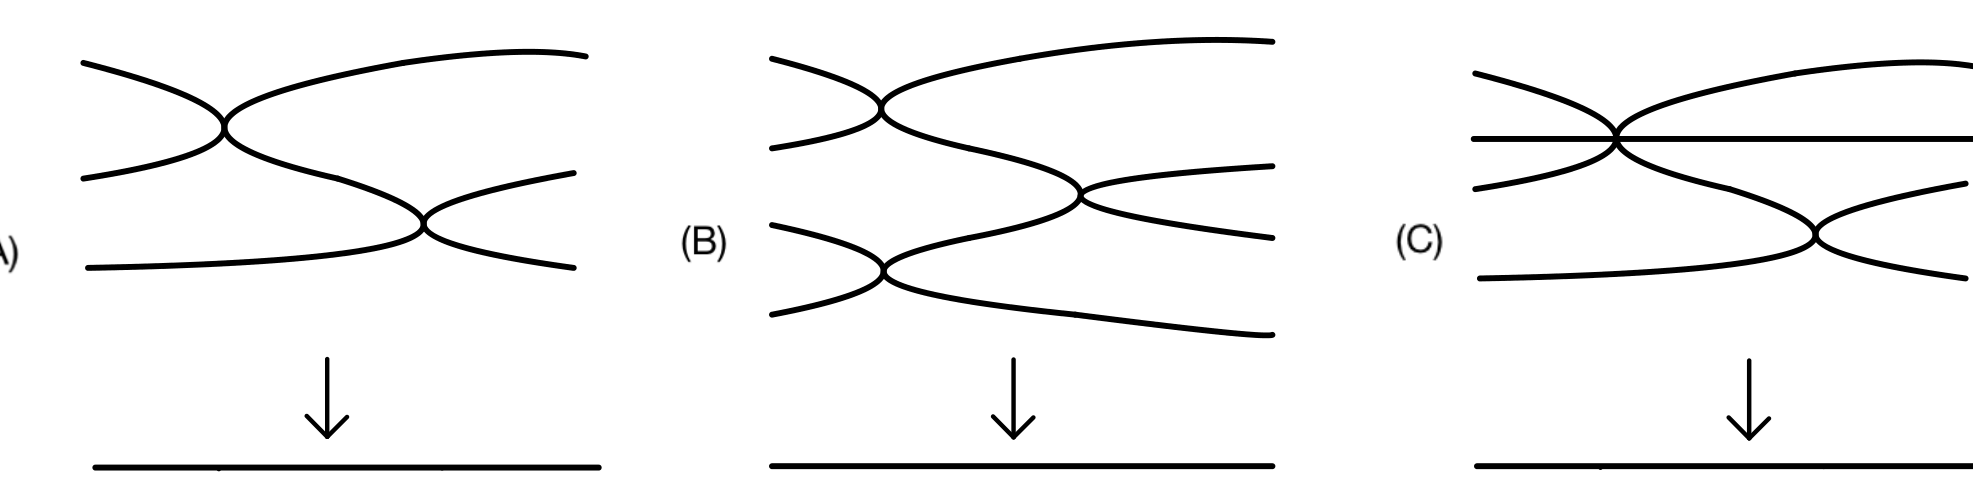
\includegraphics[width=.85\textwidth]{figures/fig-6.7.3.png}
\caption{$\mathbb P^1$ 上分歧覆盖的例子: (A) 单分歧, (B), (C) 则不是. 虽然图中源曲线 $C$ 看起来不光滑, 它在基域 $k$ 上实际上光滑. 但映射 $C\to\mathbb P^1$ 不光滑, 图示旨在反映 $C$ 在 $\mathbb P^1$ 上的奇点.}\label{src:6.7.3}\end{figure}
若 $f:C\to\allowbreak D$ 是分歧覆盖, \newterm{分歧除子}{ramification divisor} 定义为
\[
R=\sum_{p\in C(k)}\operatorname{length}(\Omega_{C/D})_p\cdot p
\overset{\text{若 }f\text{ 温和分歧}}{=}\sum_{p\in C(k)}(e_p-1).
\]
\begin{theorem}[Riemann--Hurwitz]\label{src:6.7.4}
若 $f:C\to\allowbreak D$ 是分歧除子为 $R$ 的分歧覆盖, 则 $\Omega_C\cong f^*\Omega_D\otimes\mathcal O_C(R)$, 且
\[
2g(C)-2=\deg(f)(2g(D)-2)+\deg R.
\]
特别地, 若 $f:C\to\mathbb P^1$ 单分歧, 则它在 $2g+2d-2$ 个互异点上方分歧.
\end{theorem}
\begin{proof}
直接由正合列~\bookeqref{6.7.1} 得出. 另见~\cite[命题 IV.2.3]{Har77}.
\end{proof}
\begin{example}\label{src:6.7.5}
分歧覆盖的局部模型为 $x\mapsto x^n$ 定义的 $f:\mathbb A^1\to\mathbb A^1$. 相对微分层为 $\Omega_{\mathbb A^1/\mathbb A^1}=k[x]\langle dx\rangle/(nx^{n-1}dx)$. 因而若 $\operatorname{char}(k)\nmid n$, $f$ 是在 $\mathbb A^1\setminus0$ 上平展, 在 $0$ 处以指数 $n-1$ 温和分歧的分歧覆盖.
\end{example}
\begin{exercise}\label{src:6.7.6}
证明每个分歧覆盖在指数 $n-1$ 的分歧点附近, 平展局部同构于 $\mathbb A^1\to\mathbb A^1$, $x\mapsto x^n$.
\end{exercise}
\noindent\textbf{代数, 全纯与拓扑分歧覆盖.} $\mathbb P^1$ 的全纯 (分别地, 拓扑) 分歧覆盖是非恒定全纯 (分别地, 连续) 态射 $f:C\to\mathbb P^1$, 其中 $C$ 是连通紧 Riemann 曲面 (分别地, 连通 Hausdorff 紧拓扑空间, 且 $f$ 在 $\mathbb P^1$ 的有限个点的补集上是覆盖空间).
\begin{proposition}\label{src:6.7.7}
在 $\mathbb C$ 上有自然双射
\[
\{C\to\mathbb P^1\text{ 的代数分歧覆盖}\}
\longleftrightarrow\{C\to\mathbb P^1\text{ 的全纯分歧覆盖}\}
\longleftrightarrow\{C\to\mathbb P^1\text{ 的拓扑分歧覆盖}\}.
\]
\end{proposition}
\begin{proof}
代数分歧覆盖全纯, 全纯分歧覆盖是拓扑分歧覆盖. 反之, 若 $f:C\to\mathbb P^1$ 是拓扑覆盖, 则 $\mathbb P^1$ 的全纯结构自然诱导 $C$ 的全纯结构, 使 $f$ 解析. 依赖隐函数定理的经典事实表明, 存在 $C$ 和 $\mathbb P^1$ 的局部坐标片, 使 $f$ 描述为 $z\mapsto z^k$ (参见~\cite[命题 II.4.1]{Mir95}), 这蕴涵 $C$ 代数.
\end{proof}
\noindent\textbf{单值作用.} 设 $f:C\to\mathbb P^1$ 是 $\mathbb C$ 上的 $d$ 次 (拓扑) 分歧覆盖, $B\subseteq\mathbb P^1$ 为分歧轨迹, 即使 $f^{-1}(\mathbb P^1\setminus B)\to\mathbb P^1\setminus B$ 成为覆盖空间的最小点集. 选取基点 $q\in\mathbb P^1\setminus B$. $\pi_1(\mathbb P^1\setminus B,\allowbreak q)$ 在纤维 $f^{-1}(q)$ 上的\newterm{单值作用}{monodromy action} 如下定义: 对 $\gamma\in\pi_1(\mathbb P^1\setminus B,\allowbreak q)$ 和 $p\in f^{-1}(q)$, 路径 $\gamma:[0,\allowbreak 1]\to\mathbb P^1$ 唯一提升为路径 $\widetilde\gamma:[0,\allowbreak 1]\to\allowbreak C$, 满足 $\widetilde\gamma(0)=p$, 并定义 $\gamma\cdot p=\widetilde\gamma(1)$.
\begin{figure}[H]\centering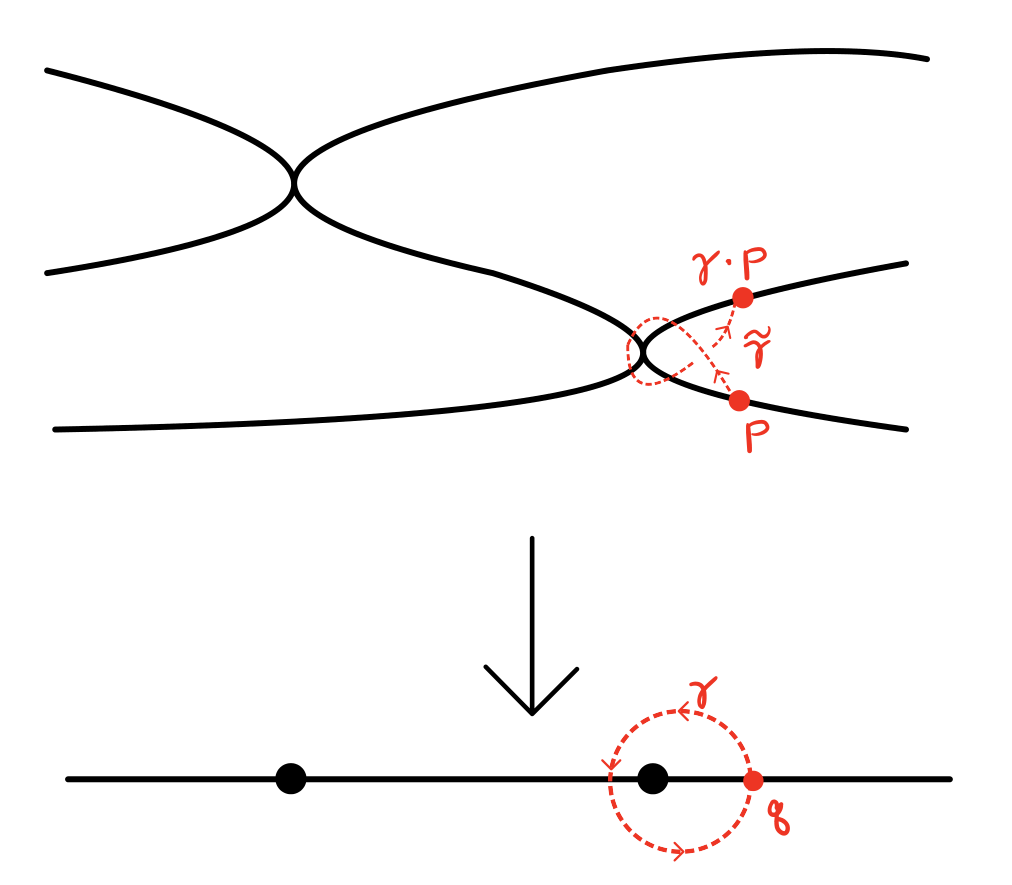
\includegraphics[width=.55\textwidth]{figures/fig-6.7.8.png}
\caption{单值作用.}\label{src:6.7.8}\end{figure}
选择双射 $f^{-1}(p)\cong\{1,\allowbreak \ldots,\allowbreak d\}$ 定义群同态 $\rho:\pi_1(\mathbb P^1\setminus B,\allowbreak q)\to\allowbreak S_d$, 称为\newterm{单值表示}{monodromy representation}. 反之, 每个这样的群同态均由分歧覆盖诱导.
\newpage
\begin{proposition}\label{src:6.7.9}
设 $B\subseteq\mathbb P^1$ 是大小 $b$ 的有限集, $q\in\mathbb P^1\setminus B$, $d>0$ 为正整数. 基本群 $\pi_1(\mathbb P^1\setminus B,\allowbreak q)$ 可认同为绕 $B$ 中各点的简单环路 $\sigma_i$ ($i=1,\allowbreak \ldots,\allowbreak b$) 生成的自由群. 有同构类的自然双射
\[
\left\{\begin{array}{l}\text{在 }B\text{ 上方单分歧的}\\d\text{ 次覆盖 }C\to\mathbb P^1\end{array}\right\}/{\sim}
\longleftrightarrow
\left\{\begin{array}{l}\rho:\pi_1(\mathbb P^1\setminus B,q)\to S_d\text{ 为群同态},\\\operatorname{im}(\rho)\subseteq S_d\text{ 是传递子群},\\\text{每个 }\rho(\sigma_i)\text{ 为对换}\end{array}\right\}/{\sim}.
\]
两个覆盖等价指它们在 $\mathbb P^1$ 上同构; 两个同态 $\rho$, $\rho'$ 等价指相差 $S_d$ 的内自同构, 即存在 $h\in S_d$ 使 $\rho'=h^{-1}\rho h$.
\end{proposition}
\begin{proof}
左到右的自然映射已说明. 反之, 给定群同态 $\rho$, 令 $H\subseteq\pi_1(\mathbb P^1\setminus B,\allowbreak q)$ 为固定 $1$ 的元素 $\gamma$ 组成的子群. 它的指数为 $d$, 因而对应于覆盖空间 $C^*\to\mathbb P^1\setminus B$, 可证其延拓为 $d$ 次有限态射 $C\to\mathbb P^1$. $C$ 连通等价于 $\operatorname{im}(\rho)$ 传递, 覆盖单分歧等价于每个 $\rho(\sigma_i)$ 为对换. 见~\cite[命题 III.4.9]{Mir95}.
\end{proof}
\subsection{Hurwitz 模空间}\label{src:6.7.2-subsection}
对正整数 $g,\allowbreak b$, 定义并研究 Hurwitz 模空间
\[
\operatorname{Hur}_{g,b}:=\{\text{在 }b\text{ 个有序点上方单分歧的亏格 }g\text{ 覆盖 }C\to\mathbb P^1\}
\]
及其与 $\mathcal M_g$ 的关系. 由 Riemann--Hurwitz (\bookref{6.7.4}), 若覆盖的次数为 $d$, 则 $b=2g+2d-2$. 文献中 Hurwitz 空间有时记作 $\operatorname{Hur}_{d,\allowbreak b}$ 或 $\operatorname{Hur}_{d,\allowbreak g}$. 关键图为
\begin{equation}\label{src:6.7.10}
\begin{tikzcd}
&\operatorname{Hur}_{g,b}\arrow[dl]\arrow[dr]&\\
\mathcal M_g&&M_{0,b},
\end{tikzcd}
\end{equation}
将单分歧覆盖映到 $C\in\mathcal M_g$ 及 $M_{0,\allowbreak b}$ 中的 $b$ 个有序分歧点.

解析地, $\mathbb C$ 上的 $\operatorname{Hur}_{g,\allowbreak b}$ 可看作使 $\operatorname{Hur}_{g,\allowbreak b}\to\allowbreak M_{0,\allowbreak b}$ 连续的最粗拓扑所赋的拓扑空间. 代数地, 仍采用函子方法定义. 概形 $S$ 上亏格 $g$, 在 $b$ 个有序点上方单分歧的 $\mathbb P^1$ 覆盖族 $(\mathcal C\to\mathcal D\to\allowbreak S,\allowbreak \sigma_i)$, 是光滑亏格 $g$ 曲线族 $\mathcal C\to\allowbreak S$ 和 $b$-点光滑亏格 $0$ 曲线族 $(\mathcal D\to\allowbreak S,\allowbreak \sigma_i)$, 配备 $S$ 上概形的 $d$ 次有限平坦态射 $\mathcal C\to\mathcal D$, 使每个几何点 $s\in S(k)$ 的 $\mathcal C_s\to\mathcal D_s\cong\mathbb P^1_k$ 在 $\sigma_1(s),\allowbreak \ldots,\allowbreak \sigma_b(s)$ 上方单分歧.
\begin{definition}[Hurwitz 函子]\label{src:6.7.11}
对正整数 $g,\allowbreak d$, 置 $b=2g+2d-2$. \newterm{Hurwitz 函子}{Hurwitz functor} 为
\[
\begin{aligned}
\operatorname{Hur}_{g,b}:\Sch&\to\Sets,\\
S&\mapsto\{\text{亏格 }g,\text{ 次数 }d\text{ 的 }\mathbb P^1\text{ 单分歧覆盖族 }(\mathcal C\to\mathcal D\to S,\sigma_i)\}/{\sim},
\end{aligned}
\]
其中两个族等价指存在同构 $\mathcal C\xrightarrow{\sim}\mathcal C'$ 和 $\mathcal D'\xrightarrow{\sim}\mathcal D'$, 与截面和结构态射 $\mathcal C\to\mathcal D$, $\mathcal C'\to\mathcal D'$ 相容.
\end{definition}
有叠的态射 $\operatorname{Hur}_{g,\allowbreak b}\to\mathcal M_g$ 和 $\operatorname{Hur}_{g,\allowbreak b}\to\allowbreak M_{0,\allowbreak b}$, 分别取覆盖族的 $\mathcal C\to\allowbreak S$ 和 $(\mathcal D\to\allowbreak S,\allowbreak \sigma_i)$, 给出图~\bookeqref{6.7.10}.
\begin{remark}[变体]\label{src:6.7.12}
文献中也将上述定义的若干变体称为 Hurwitz 模空间. 首先可刚化模问题, 考虑函子 $\operatorname{Hur}_{g,\allowbreak b}^{\mathrm{rig}}:\Sch\to\allowbreak S$, 在 $S$ 上的对象是从光滑亏格 $g$ 曲线族出发的 $S$ 上有限平坦态射 $\mathcal C\to\mathbb P^1_S$, 配备互不相交的有序截面 $\sigma_1,\allowbreak \ldots,\allowbreak \sigma_b:S\to\mathbb P^1_S$, 使每个几何纤维在这些截面所给点上方单分歧. 两个族等价指它们在 $\mathbb P^1_S$ 上同构且截面相等. 有态射 $\operatorname{Hur}_{g,\allowbreak b}^{\mathrm{rig}}\to(\mathbb P^1)^b\setminus\Delta$, 其中 $\Delta$ 是所有两两对角线的并. 代数群 $\operatorname{PGL}_2$ 自由作用于 $\operatorname{Hur}_{g,\allowbreak b}^{\mathrm{rig}}$, 商可认同为 $\operatorname{Hur}_{g,\allowbreak b}$, 等变态射 $\operatorname{Hur}_{g,\allowbreak b}^{\mathrm{rig}}\to(\mathbb P^1)^b\setminus\Delta$ 的商则认同为 $\operatorname{Hur}_{g,\allowbreak b}\to\allowbreak M_{0,\allowbreak b}$.

另一常见变体是将分歧轨迹看作无序点集, 这是 Hurwitz 在~\cite{Hur91} 中最初考虑的版本. 函子 $\operatorname{Hur}_{g,\allowbreak b}^{\mathrm{rig,\allowbreak unord}}:\Sch\to\Sets$ 的 $S$ 上对象是从光滑亏格 $g$ 曲线族出发的有限平坦态射 $f:\mathcal C\to\mathbb P^1_S$, 使每个几何纤维为在 $b$ 个点上方单分歧的覆盖. 断言有到参数化 $b$ 个无序互异点的空间的态射 $\operatorname{Hur}_{g,\allowbreak b}^{\mathrm{rig,\allowbreak unord}}\to\operatorname{Sym}^b\mathbb P^1\setminus\Delta$. 事实上, 由 $f$ 的相对奇点轨迹定义的分歧除子 $R_f\subseteq\mathcal C$ 在 $S$ 上有限平展, 次数为 $b=2g+2d-2$. 两两对角线的补集 $R_f\times_S\cdots\times_S R_f\setminus\Delta$ 是 $S$ 上的主 $S_b$-挠子 (见习题~\bookref{B.1.55}), 到 $\mathbb P^1_S\times_S\cdots\times_S\mathbb P^1_S\setminus\Delta$ 的映射为 $S_b$-等变. 它定义商叠 $[((\mathbb P^1)^b\setminus\Delta)/S_b]$ 的 $S$-值点, 该商叠可认同为概形 $\operatorname{Sym}^b\mathbb P^1\setminus\Delta$. 还有 $\operatorname{Sym}^b\mathbb P^1\setminus\Delta\cong\mathbb P^b\setminus\Delta$, 后一 $\Delta$ 为判别式超曲面. 对称群 $S_b$ 自由作用于 $\operatorname{Hur}_{g,\allowbreak b}^{\mathrm{rig}}$, 商为 $\operatorname{Hur}_{g,\allowbreak b}^{\mathrm{rig,\allowbreak unord}}$; 相应态射的 $S_b$-商可认同为 $\operatorname{Hur}_{g,\allowbreak b}^{\mathrm{rig,\allowbreak unord}}\to\operatorname{Sym}^b\mathbb P^1\setminus\Delta$.
\end{remark}
下列习题保证 $\operatorname{Hur}_{g,\allowbreak b}\to\allowbreak M_{0,\allowbreak b}$ 有限, 平展且满射, 即代数覆盖空间. 在域 $k$ 上工作时, 也用 $\operatorname{Hur}_{g,\allowbreak b}$ 表示基变换 $\operatorname{Hur}_{g,\allowbreak b}\times_{\mathbb Z}k$.
\begin{exercise}\label{src:6.7.13}
设 $k$ 是特征 $0$ 的代数闭域, $g,\allowbreak b,\allowbreak d$ 是正整数, $b=2g+2d-2$, $d>2$.
\begin{enumerate}[(a)]
\item 证明 $\operatorname{Hur}_{g,\allowbreak b}$ 在 $k$ 上的对角线由概形可表.
\item 若 $\mathcal C\to\mathbb P^1_k$ 是 $d$ 次单分歧覆盖, 证明 $\mathcal C$ 在 $\mathbb P^1$ 上的每个自同构平凡. 推出 $d$ 次 $\mathbb P^1$ 单分歧覆盖族的自同构群概形也平凡.

提示: 用光滑曲线固定超过 $2g+2$ 个点的自同构必平凡 (习题~\bookref{6.1.9}).
\item (困难) 证明 $\operatorname{Hur}_{g,\allowbreak b}\to\allowbreak M_{0,\allowbreak b}$ 是有限平展可表态射. 特别地, Hurwitz 函子由概形可表. 另见~\cite[定理 7.2]{Ful69}, 其中更一般地证明了它在 $\Spec\mathbb Z$ 上可表, 且该映射平展 (在特征大于 $d$ 的基底上有限平展).
\item 验证注记~\bookref{6.7.12} 中两个刚化函子也由概形可表.
\end{enumerate}
\end{exercise}
\begin{remark}\label{src:6.7.14}
下一节证明 Clebsch--Hurwitz--Lüroth 定理 (\bookref{6.7.19}) 时, 只需知道 $\operatorname{Hur}_{g,\allowbreak b}\to\allowbreak M_{0,\allowbreak b}$ 是拓扑覆盖空间, 这有初等论证. 参照图~\bookref{6.7.15}, 给定单分歧覆盖 $f:C\to\mathbb P^1$ 和分歧点 $p\in C$, 可在 $f(p)$ 附近取开邻域 $U\subseteq\mathbb P^1$, 使 $f^{-1}(U)\to\allowbreak U$ 同构于 $x\mapsto x^n$ 给出的 $\mathbb C\to\mathbb C$ 的开邻域. 对每个 $q'\in U$, 可构造分歧覆盖 $C'\to\mathbb P^1$, 在 $U$ 外与原覆盖相同, 在 $U$ 上局部同构于 $x\mapsto x^n$, 但以 $q'$ 而非 $f(p)$ 为中心.
\end{remark}
\begin{figure}[H]\centering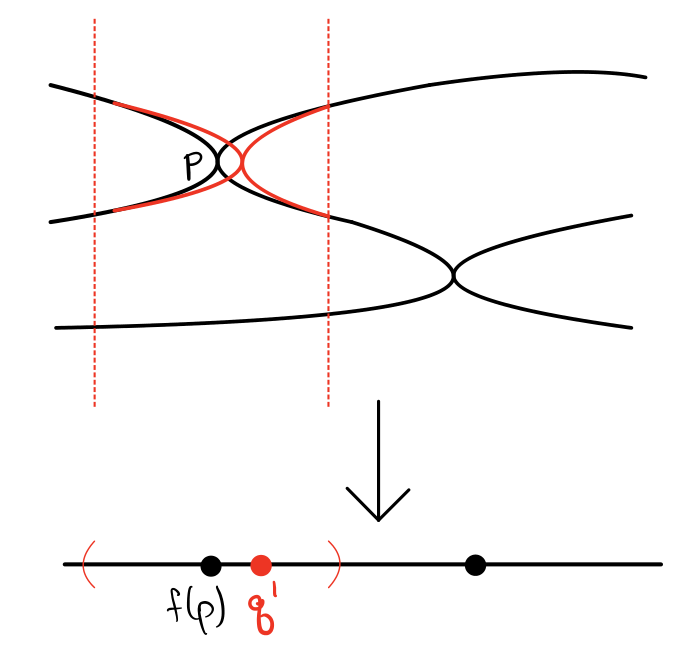
\includegraphics[width=.35\textwidth]{figures/fig-6.7.15.png}
\caption{}\label{src:6.7.15}\end{figure}
现在研究另一映射 $\operatorname{Hur}_{g,\allowbreak b}\to\mathcal M_g$.
\newpage
\begin{lemma}\label{src:6.7.16}
设 $C$ 是特征 $0$ 代数闭域 $k$ 上光滑, 连通, 亏格 $g$ 的射影曲线. 若 $L$ 是次数 $d\geq2g+3$ 的线丛, $V\subseteq\mathrm H^0(C,\allowbreak L)$ 是维数为 $2$ 的线性系, 则选择 $V$ 的基诱导单分歧覆盖 $C\to\mathbb P^1$.
\end{lemma}
\begin{proof}
作维数计算. 因为 $\deg(\omega_C\otimes L^\vee)<0$, 有 $\mathrm h^1(C,\allowbreak L)=\mathrm h^0(C,\allowbreak \omega_C\otimes L^\vee)=0$. Riemann--Roch 给出 $\mathrm h^0(C,\allowbreak L)=d+1-g$, 所以 $2$ 维子空间的 Grassmann 簇 $\operatorname{Gr}(2,\allowbreak \mathrm H^0(L))$ 的维数为 $2(d-g-1)$. 因为 $\operatorname{char}(k)=0$, 每个有限态射 $C\to\mathbb P^1$ 自动可分. 若 $V$ 不诱导单分歧覆盖, 则必满足下列条件之一:
\begin{enumerate}[(a)]
\item $V$ 有基点;
\item 存在分歧指数大于 $2$ 的分歧点;
\item 同一纤维中有两个分歧点.
\end{enumerate}
断言各条件均为余维至少一的闭条件. 对 (a), 若 $p\in C(k)$ 是基点, 则 $V\subseteq\mathrm H^0(C,\allowbreak L(-p))$. 由 $d\geq2g$, 有 $\deg(\omega_C\otimes(L(-p))^\vee)<0$, 因而 $\mathrm h^0(C,\allowbreak L(-p))=d-g$, $\dim\operatorname{Gr}(2,\allowbreak \mathrm H^0(C,\allowbreak L(-p)))=2(d-g-2)$. 让 $p\in C$ 变化, (a) 定义的轨迹维数为 $2(d-g-2)+1=\dim\operatorname{Gr}(2,\allowbreak \mathrm H^0(L))-1$. (b), (c) 留给读者. 另见~\cite{Sev21} 和~\cite[命题 8.1]{Ful69}.
\end{proof}
\begin{exercise}[细节]\label{src:6.7.17}
\begin{enumerate}[(a)]
\item 验证上述 (b), (c) 为余维至少一的闭条件.
\item 证明只要 $\operatorname{char}(k)\ne2$, 论证仍成立, 并说明在特征 $2$ 时为何失效.
\end{enumerate}
\end{exercise}
\begin{corollary}\label{src:6.7.18}
设 $k$ 是特征 $0$ 的代数闭域. 若 $g\geq2$, $d\geq2g+3$, $b=2g+2d-2$, 则态射 $\operatorname{Hur}_{g,\allowbreak b}\to\mathcal M_g$, $(C\to\mathbb P^1,\allowbreak \sigma_i)\mapsto C$ 满射.
\end{corollary}
\subsection{Clebsch--Hurwitz--Lüroth 定理}\label{src:6.7.3-subsection}
给出 Clebsch~\cite{Cle73}, Hurwitz~\cite{Hur91} 和 Lüroth~\cite{Lür71} 证明 $\mathbb C$ 上 Hurwitz 模空间连通的经典论证. 由 $\operatorname{Hur}_{g,\allowbreak b}\to\mathcal M_g$ 满射, 推出 $\mathcal M_g$ 不可约, 这是 Klein~\cite[\S19]{Kle82} 和 Severi~\cite[\S F]{Sev21} 的经典结果. 现代论述见~\cite[命题 1.5]{Ful69}.
\begin{theorem}[Clebsch--Hurwitz--Lüroth 定理]\label{src:6.7.19}
若 $g\geq2$, $d\geq2$, $b=2g+2d-2$, 则 $\mathbb C$ 上的 Hurwitz 模空间 $\operatorname{Hur}_{g,\allowbreak b}$ 连通.
\end{theorem}
\begin{proof}
利用将单分歧覆盖映为有序分歧轨迹的态射 $\beta:\operatorname{Hur}_{g,\allowbreak b}\to\allowbreak M_{0,\allowbreak b}$. 由习题~\bookref{6.7.13}(c), 这是覆盖空间. 对有序互异点集 $B=\{q_1,\allowbreak \ldots,\allowbreak q_b\}\subseteq\mathbb P^1$ 及 $q\in\mathbb P^1\setminus B$, 基本群 $\pi_1(\mathbb P^1\setminus B,\allowbreak q)=\langle\sigma_i\mid\sigma_1\cdots\sigma_b=1\rangle$ 作用于单分歧覆盖 $f:C\to\mathbb P^1$ 的纤维 $f^{-1}(p)$, 其中 $\sigma_i$ 绕 $q_i$ 一周. 同样, 因为 $\beta$ 是覆盖空间, $\pi_1(M_{0,\allowbreak b},\allowbreak B)$ 作用于纤维 $\operatorname{Hur}_{d,\allowbreak B}:=\beta^{-1}(B)\subseteq\operatorname{Hur}_{g,\allowbreak b}$. (注意大写下标 $B$ 与小写 $b$ 的区别.) 由命题~\bookref{6.7.9}, 有双射
\[
\begin{aligned}
\operatorname{Hur}_{g,B}
&=\{\text{在 }B\text{ 上方单分歧的亏格 }g\text{ 覆盖 }C\to\mathbb P^1\}/{\sim}\\
&\cong\left\{\begin{array}{l}\text{群同态 }\rho:\pi_1(\mathbb P^1\setminus B,q)\to S_d,\\\operatorname{im}(\rho)\text{ 传递, 每个 }\rho(\sigma_i)\text{ 为对换}\end{array}\right\}/S_d\text{ 共轭}\\
&\cong\left\{\begin{array}{l}\text{对换序列 }(\tau_1,\ldots,\tau_b)\in(S_d)^b,\\\text{乘积为 }1,\text{ 生成传递子群}\end{array}\right\}/S_d\text{ 共轭}.
\end{aligned}
\]
Hurwitz 空间连通等价于 $\pi_1(M_{0,\allowbreak b},\allowbreak B)$ 在纤维 $\operatorname{Hur}_{d,\allowbreak B}$ 上的作用传递. 考虑序列
\[
\tau=\bigl(\underbrace{(12),(12),(13),(13),\ldots,(1\ d-1),(1\ d-1)}_{2(d-2)},
\underbrace{(1d),(1d),\ldots,(1d)}_{2g+2}\bigr)\in\operatorname{Hur}_{d,B}.
\]
只需证明每个轨道包含 $\tau$. 为此定义环路
\[
\begin{aligned}
\Gamma_i:[0,1]&\to M_{0,b},\\
t&\mapsto(q_1,\ldots,q_{i-1},\gamma_i(t),\gamma'_i(t),q_{i+2},\ldots,q_b),
\end{aligned}
\]
其中 $\gamma_i$, $\gamma'_i$ 如图~\bookref{6.7.20}.
\begin{figure}[H]\centering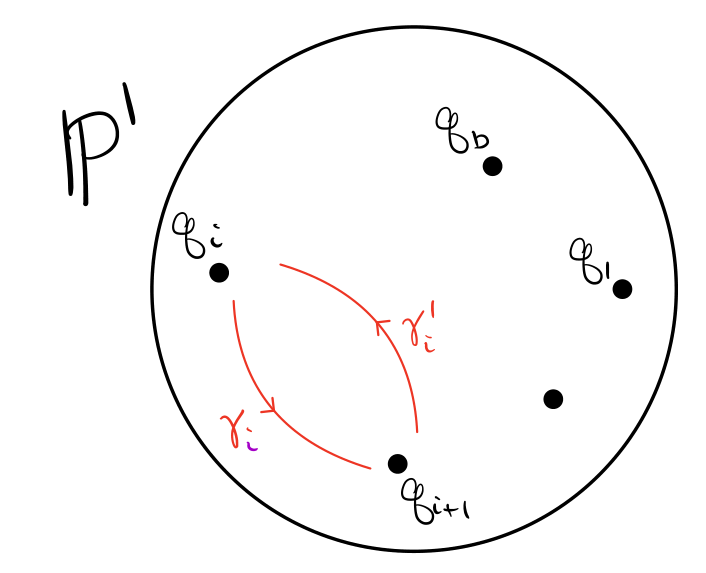
\includegraphics[width=.35\textwidth]{figures/fig-6.7.20.png}
\caption{$\mathbb P^1$ 中的路径.}\label{src:6.7.20}\end{figure}
对 $(\lambda_1,\allowbreak \ldots,\allowbreak \lambda_b)\in\operatorname{Hur}_{g,\allowbreak b}$, $\Gamma_i$ 的作用为
\[
\Gamma_i\cdot(\lambda_1,\ldots,\lambda_b)
=(\lambda_1,\ldots,\lambda_{i-1},\lambda_{i-1}^{-1}\lambda_{i+1}\lambda_i,\lambda_i,\lambda_{i+2},\ldots,\lambda_b).
\]
剩下是组合问题: 证明存在环路序列 $\Gamma_{i_1},\allowbreak \ldots,\allowbreak \Gamma_{i_k}$, 使 $\tau=\Gamma_{i_1}\Gamma_{i_2}\cdots\Gamma_{i_k}\cdot(\lambda_1,\allowbreak \ldots,\allowbreak \lambda_b)$. 留给读者.
\end{proof}
\begin{exercise}\label{src:6.7.21}
解决上述证明末尾的组合问题.
\end{exercise}
\begin{corollary}[$\mathcal M_g$ 的不可约性]\label{src:6.7.22}
对任意特征 $0$ 域 $k$, $\mathcal M_g$ 不可约.
\end{corollary}
\begin{proof}
由 $\operatorname{Hur}_{g,\allowbreak b}\to\mathcal M_g$ 满射 (推论~\bookref{6.7.18}), Hurwitz 空间在 $\mathbb C$ 上连通蕴涵 $\mathcal M_g$ 在 $\mathbb C$ 上连通. 因而 $\mathcal M_g$ 在 $\mathbb Q$ 上几何连通, 在任意特征 $0$ 域 $k$ 上连通. 又因 $\mathcal M_g$ 光滑 (定理~\bookref{6.4.16}), 连通性等价于不可约性.
\end{proof}
还可用参数化亏格 $g$ 拓扑曲面 $\Sigma_g$ 上复结构的 Teichmüller 空间 $\mathcal T_g$ 建立不可约性. \cite{Ber60} 首次证明 $\mathcal T_g$ 同胚于 $\mathbb C^{3g-3}$ 中的球, 且 $\mathcal M_g$ 可认同为对映射类群 $\Gamma_g$ 的商 $\mathcal T_g/\Gamma_g$.
\subsection{通过退化证明不可约性}\label{src:6.7.4-subsection}
现在给出特征 $0$ 下 $\mathcal M_g$ 不可约的纯代数论证. 关键是证明每条光滑曲线退化为有奇点的稳定曲线 (命题~\bookref{6.7.26}); 这是最困难的部分, 所用技术受到容许覆盖理论的启发. 由此将连通性归结为边界 $\delta=\overline{\mathcal M}_g\setminus\mathcal M_g$ 的连通性, 再利用归纳结构与粘合态射 (\bookref{6.6.16}) 建立后者. 此论证与 Deligne 和 Mumford 对正特征下 $\overline M_g$ 不可约性的第一个证明精神相近 (见注记~\bookref{6.7.34}). 遵循 Harris 和 Mumford 论文中 Fulton 所写附录~\cite{HM82} 的论述.

先热身, 考虑亏格 $0$.
\begin{proposition}\label{src:6.7.23}
对每个代数闭域 $k$ 和每个整数 $n\geq3$, $\overline M_{0,\allowbreak n}$ 不可约.
\end{proposition}
\begin{proof}
因为 $\overline M_{0,\allowbreak n}$ 光滑, 只需证连通. $M_{0,\allowbreak n}$ 可认同为 $(\mathbb P^1\setminus\{0,\allowbreak 1,\allowbreak \infty\})^{n-3}\setminus\Delta$, 其中 $\Delta$ 为两两对角线的并 (见习题~\bookref{4.1.22}), 故连通. 只需证边界无完全由有奇点曲线组成的连通分支. 给定 $(C,\allowbreak p_i)\in\overline M_{0,\allowbreak n}(k)$ 有奇点, 容易直接构造离散赋值环 $R$ 上的稳定族 $(\mathcal C\to\Spec R,\allowbreak \sigma_i)$, 一般纤维光滑, 特殊纤维为 $(C,\allowbreak p_i)$. 事实上, $C$ 的每个结点有形如 $\Spec k[x,\allowbreak y]/(xy)$ 的 Zariski 开邻域, 可将 $\Spec k[x,\allowbreak y]/(xy-\pi)$ 的形变粘为族, $\pi\in R$ 为一致化参数. 或者由形变理论命题~\bookref{6.3.26}, 有相容稳定族 $(\mathcal C_n\to\Spec k[t]/(t^{n+1}),\allowbreak \sigma_{n,\allowbreak i})$, $(\mathcal C_0,\allowbreak \sigma_{0,\allowbreak i})=(C,\allowbreak p_i)$, 由 Grothendieck 存在定理 (\bookref{C.5.8}) 有效化为一般纤维光滑的稳定族 $(\mathcal C\to\Spec k[[t]],\allowbreak \sigma_i)$.

另一证明采用稍后证明 $\overline{\mathcal M}_{g,\allowbreak n}$ 连通的同一策略. 先断言 $n$-点曲线 $(\mathbb P^1,\allowbreak p_i)$ 在单参数族中退化为有奇点的 $n$-点稳定曲线. 让 $p_1$, $p_2$ 以不同速度趋近, 爆破中心纤维中的交点, 总族与截面的严格变换便给出中心纤维有奇点的 $n$-点稳定亏格 $0$ 曲线族. 因而只需证边界 $\delta=\overline M_{0,\allowbreak n}\setminus M_{0,\allowbreak n}$ 连通. 它分解为
\[
\delta=\bigcup_I\delta_{0,I},\qquad
\delta_{0,I}=\operatorname{im}(\overline{\mathcal M}_{0,I\cup\{p\}}\times\overline{\mathcal M}_{0,I^c\cup\{q\}}\to\overline{\mathcal M}_{0,n}),
\]
其中 $2\leq|I|\leq n-2$, 且 $\delta_{0,\allowbreak I}=\delta_{0,\allowbreak I^c}$. 由归纳, 可假设 $k<n$ 时 $\overline M_{0,\allowbreak k}$ 不可约; 初始情形由 $\overline M_{0,\allowbreak 3}=\Spec k$ 成立. 故每个 $\delta_{0,\allowbreak I}$ 连通. 给定不同子集 $I,\allowbreak J$, 必要时将 $I$ 换为 $I^c$, 可假设 $K:=I\cap J$ 至少有两个元素. 若 $K\subsetneq I$, $K\subsetneq J$, 图~\bookref{6.7.24} 给出 $\delta_{0,\allowbreak I}\cap\delta_{0,\allowbreak K}\ne\varnothing$, $\delta_{0,\allowbreak J}\cap\delta_{0,\allowbreak K}\ne\varnothing$. 若 $I\subseteq J$ 或 $J\subseteq I$, 同理 $\delta_{0,\allowbreak I}\cap\delta_{0,\allowbreak J}\ne\varnothing$. 因而 $\delta$ 连通.
\end{proof}
\begin{figure}[H]\centering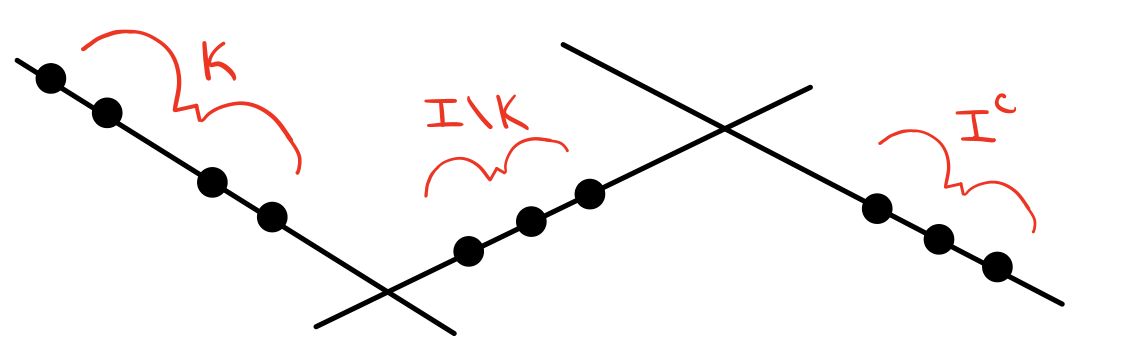
\includegraphics[width=.6\textwidth]{figures/fig-6.7.24.png}
\caption{只要 $K\subsetneq I$, 图中曲线就属于 $\delta_{0,\allowbreak I}\cap\delta_{0,\allowbreak K}$.}\label{src:6.7.24}\end{figure}
\begin{exercise}\label{src:6.7.25}
证明代数闭域 $k$ 上每条稳定曲线 $C$ 可形变为光滑曲线. 更精确地, 存在 $k$ 上连通曲线\footnote{依照约定, 曲线 (定义~\bookref{6.1.1}) 必在 $k$ 上有限型.} $T$ 上的稳定曲线族 $\pi:\mathcal C\to\allowbreak T$ 及点 $t\in T(k)$, 使 $\mathcal C_t\cong C$, $\pi^{-1}(T\setminus\{t\})\to\allowbreak T\setminus\{t\}$ 光滑.
\end{exercise}
逆命题, 即每条光滑曲线退化为稳定曲线, 更难.
\begin{proposition}\label{src:6.7.26}
设 $C$ 是特征 $0$ 代数闭域 $k$ 上光滑, 连通, 亏格 $g\geq2$ 的射影曲线. 则存在 $k$ 上光滑连通曲线 $T$ 上的稳定曲线族 $\mathcal C\to\allowbreak T$, 以及点 $s,\allowbreak t\in T(k)$, 使 $\mathcal C_s\cong C$, $\mathcal C_t$ 是有奇点的稳定曲线.
\end{proposition}
\begin{proof}
基本策略如下:
\begin{enumerate}[(1)]
\item 对 $d\gg0$, 选取 $d$ 次单分歧覆盖 $C\to\mathbb P^1$, 在互异点 $q_1,\allowbreak \ldots,\allowbreak q_b$ 上方分歧, $b=2g+2d-2$.
\item 将在 $q_i$ 上方分歧的覆盖形变为在一般点 $q'_i$ 上方分歧的 $C'\to\mathbb P^1$.
\item 将 $(\mathbb P^1,\allowbreak q'_i)\in M_{0,\allowbreak b}$ 退化为图~\bookref{6.7.27} 的稳定曲线 $(D,\allowbreak d_i)\in\overline M_{0,\allowbreak b}$.
\item 将覆盖 $C'\to\mathbb P^1$ 退化为在 $d_i$ 上方分歧的覆盖 $C''\to\allowbreak D$, 使 $C''$ 有奇点且稳定.
\end{enumerate}
\begin{figure}[H]\centering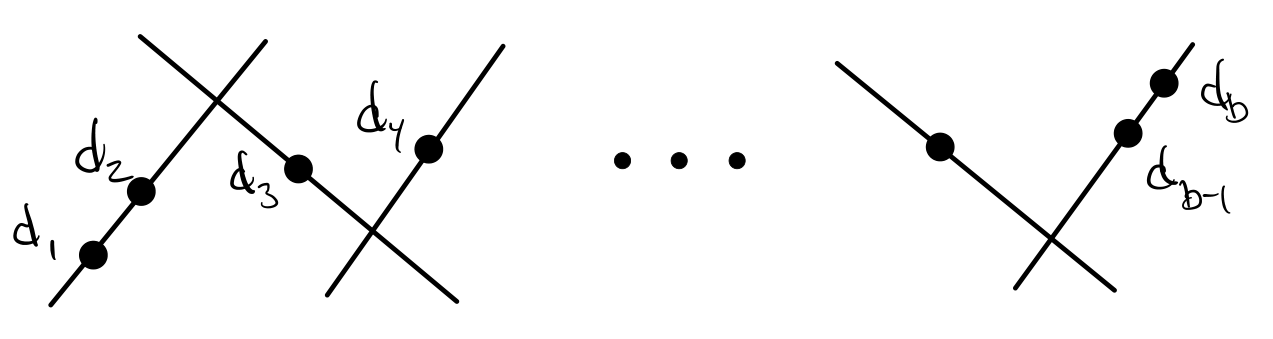
\includegraphics[width=.65\textwidth]{figures/fig-6.7.27.png}
\caption{退化曲线 $(D,\allowbreak d_i)\in\overline M_{0,\allowbreak b}$.}\label{src:6.7.27}\end{figure}
步骤 $1$ 的存在性由引理~\bookref{6.7.16} 保证, 并定义 $b$-点稳定曲线 $(\mathbb P^1,\allowbreak q_i)\in M_{0,\allowbreak b}$. 对其余步骤, 先断言只需在 $k$ 上有限型连通概形 $T$ 上找到族 $\mathcal C\to\allowbreak T$. 这表明 $C$ 与有奇点稳定曲线 $C''$ 位于 $\overline{\mathcal M}_g$ 的同一连通 (因而不可约) 分支 $\mathcal M'$. 由 Gabber 引理 (\bookref{5.6.1}), 有概形的有限覆盖 $Z\to\overline{\mathcal M}_g$, 且 $Z$ 有一个不可约分支 $Z'$ 满射到 $\mathcal M'$. $k$ 上有限型不可约概形 $Z'$ 的任意两个 $k$-点包含于整曲线 $Q\subseteq Z'$, 故考虑从 $Q$ 的正规化出发的 $\widetilde Q\to\allowbreak Z'\to\overline{\mathcal M}_g$ 即证断言.

步骤 $2$ 中, 令 $H\subseteq\operatorname{Hur}_{g,\allowbreak b}$ 为包含 $C\to\mathbb P^1$ 的连通分支. 因为 $\operatorname{Hur}_{g,\allowbreak b}\to\allowbreak M_{0,\allowbreak b}$ 有限平展 (习题~\bookref{6.7.13}(c)), 既开又闭, 复合 $H\hookrightarrow\operatorname{Hur}_{d,\allowbreak b}\to\allowbreak M_{0,\allowbreak b}$ 满射. $H$ 连通, 所以只需找到一个 $(C'\to\mathbb P^1)\in H$ 以及将 $C'$ 连到有奇点稳定曲线的连通基底上的稳定曲线族.

步骤 $3$: 断言存在交换图
\begin{equation}\label{src:6.7.28}
\begin{tikzcd}
T\setminus\{t\}\arrow[d]\arrow[r]&H\arrow[r,hook,"\text{开且闭}"]\arrow[dr]&\operatorname{Hur}_{g,b}\arrow[d,"\text{有限平展}"]\\
T\arrow[r,"{t\mapsto(D,d_i)}"']&\overline M_{0,b}&M_{0,b}\arrow[l,hook]
\end{tikzcd}
\end{equation}
其中 $T$ 光滑连通, $t$ 映到图~\bookref{6.7.27} 的稳定曲线. 因为 $\overline M_{0,\allowbreak b}$ 不可约 (命题~\bookref{6.7.23}), $M_{0,\allowbreak b}$ 稠密. 可选连通约化曲线的映射 $Y\to\overline M_{0,\allowbreak b}$ 及点 $y\in Y(k)$, 使 $y\mapsto(D,\allowbreak d_i)$, 每个其他点映到光滑曲线. 令 $Y'$ 为 $(Y\setminus\{y\})\times_{M_{0,\allowbreak b}}H$ 的连通分支, $T$ 为 $Y'\to\overline M_{0,\allowbreak b}$ 的像的闭包的正规化. 有 $t\in T$ 映到 $(D,\allowbreak d_i)$; 将 $T$ 换为 $t$ 的开邻域后, 可使 $T\setminus\{t\}\to\overline M_{0,\allowbreak b}$ 经过 $H$ 分解.

图~\bookeqref{6.7.28} 给出 $b$-点稳定亏格 $0$ 曲线族 $(\mathcal D\to\allowbreak T,\allowbreak \tau_i)$ 和 $T^*:=T\setminus\{t\}$ 上的单分歧覆盖 $\mathcal C^*\to\mathcal D^*$, 其中 $\mathcal D^*$ 为 $T^*$ 的原像, 截面 $\tau_i^*$ 选出分歧轨迹. 断言将 $(T,\allowbreak t)$ 换为分歧覆盖后, 存在虚线箭头补全 Cartesian 图
\[
\begin{tikzcd}
\mathcal C^*\arrow[r]\arrow[d,dashed]&\mathcal D^*\arrow[r]\arrow[d]&T^*\arrow[d]\\
\mathcal C\arrow[r,dashed,"f"']\arrow[ur,phantom,"\square"]&\mathcal D\arrow[r]\arrow[ur,phantom,"\square"]&T,
\end{tikzcd}
\]
其中 $\mathcal C\to\allowbreak T$ 是结点曲线族. 将 $\mathcal C$ 定义为 $\mathcal O_{\mathcal D}$ 在 $K(\mathcal C^*)$ 中的整闭包, 则 $f:\mathcal C\to\mathcal D$ 有限. 令 $\mathcal D^{\mathrm{sm}}=\mathcal D\setminus\{d_i\}$ 为相对光滑轨迹, 分歧轨迹的纯性 (\bookref{A.3.13}) 保证 $f^{-1}(\mathcal D^{\mathrm{sm}})\to\mathcal D^{\mathrm{sm}}$ 的分歧轨迹是除子. 因而 $\mathcal C\to\mathcal D$ 只在 $\tau_1,\allowbreak \ldots,\allowbreak \tau_b$ 以及可能在 $D=\mathcal D_t$ 的结点 $d_i$ 上方分歧. 为证 $\mathcal C\to\allowbreak S$ 为结点族, 注意在每个 $d_i$ 附近平展局部, 该映射形如有限态射 $U\to\allowbreak V:=\Spec k[x,\allowbreak y]/(xy-\pi^k)$, 其中 $k\leq d$, $\pi$ 是 $t\in T$ 的平展邻域上的局部坐标. $U\to\allowbreak V$ 在 $V\setminus0$ 上有限平展. 因为由 $(x',\allowbreak y')\mapsto(x'^k,\allowbreak y'^k)$ 定义的
\[
\Spec k[x',y']/(x'^ky'^k-\pi^k)\setminus0\to V\setminus0
\]
是泛覆盖, $V\setminus0$ 在 $U$ 中的原像必同构于 $\Spec k[x'',\allowbreak y'']/(x''^ly''^l-\pi^k)\setminus0$, 其中 $l\mid k$. 所以 $U=\Spec k[x'',\allowbreak y'']/(x''^ly''^l-\pi^k)$, 纤维 $U_t$ (由 $\pi=0$ 定义) 的约化概形结构仅有结点. 从而 $(\mathcal C_t)_{\mathrm{red}}$ 仅有结点. 用稳定约化 (\bookref{6.5.1}) 证明步骤 $4$ 的同一论证, 有分歧覆盖 $T'\to\allowbreak T$, 使 $\mathcal C'=\mathcal C\times_T T'$ 的正规化 $\widetilde{\mathcal C}'$ 的中心纤维约化且仅有结点. 将 $\mathcal C$ 换为 $\widetilde{\mathcal C}'$, $T$ 换为 $T'$, 便使 $\mathcal C\to\allowbreak T$ 成为结点曲线族.
\begin{figure}[H]\centering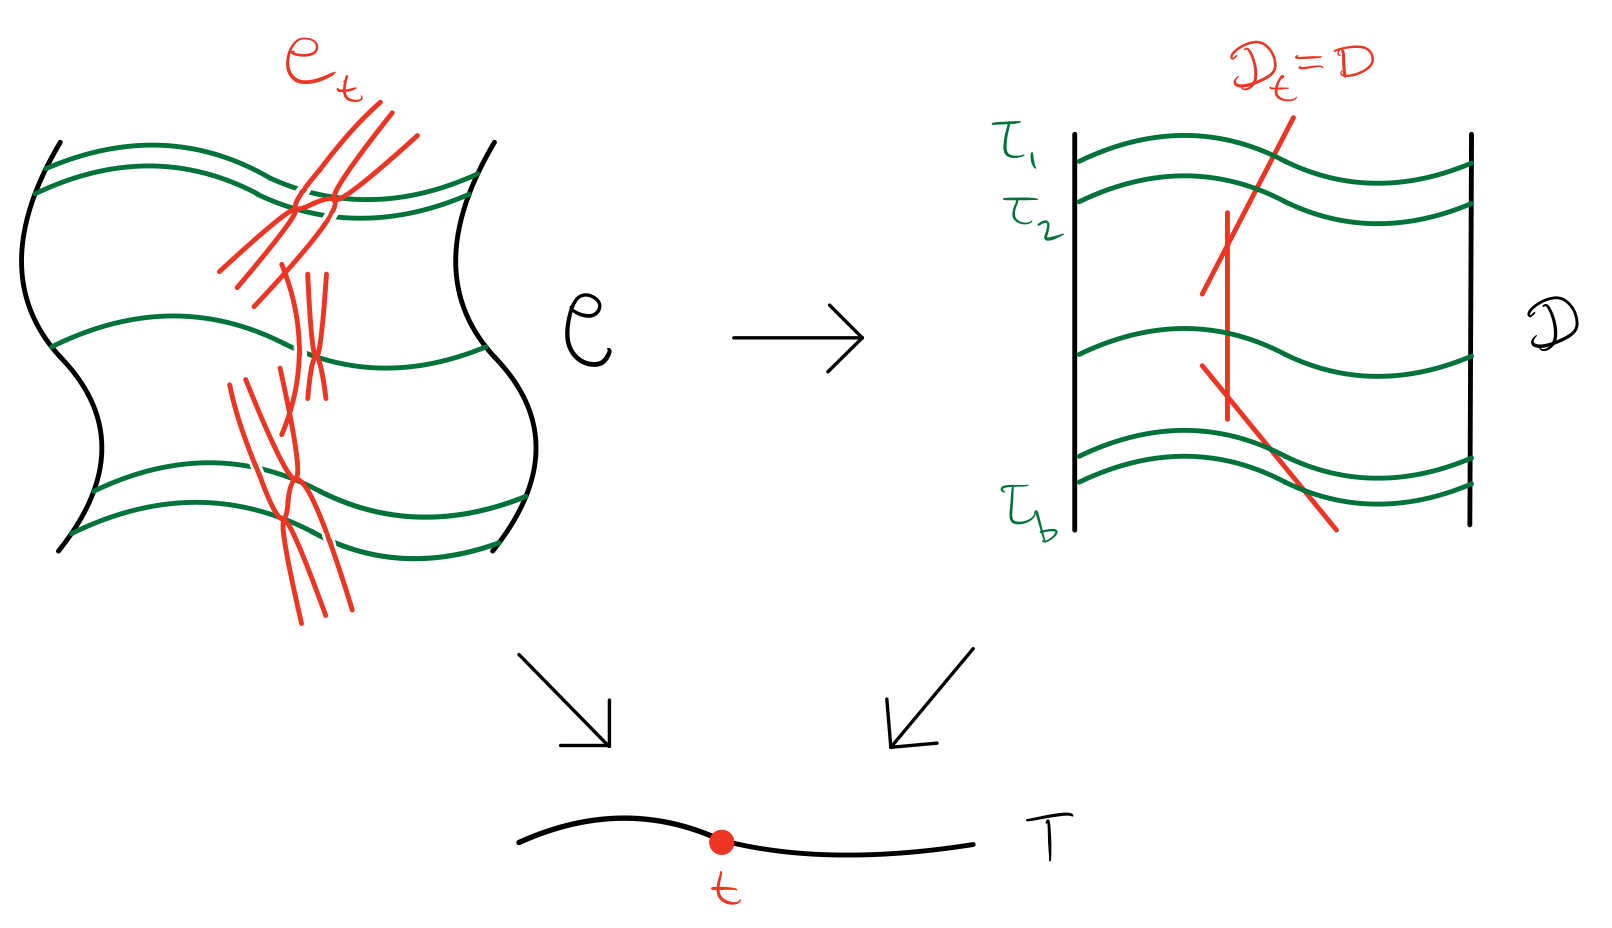
\includegraphics[width=.7\textwidth]{figures/fig-6.7.29.png}
\caption{$\mathcal C\to\mathcal D\to\allowbreak T$ 的示意图.}\label{src:6.7.29}\end{figure}
此族可能不稳定, 但由预稳定族的稳定收缩 (定理~\bookref{6.6.6}), 收缩有理尾和有理桥得到稳定族 $\mathcal C^{\mathrm{st}}\to\allowbreak T$. 为证 $C_0^{\mathrm{st}}$ 有奇点, 只需证 $C_0$ 的每个光滑不可约分支亏格为 $0$. 设 $X\subseteq C_0$ 为此分支, 它在 $C_0\to\mathcal D_0=D$ 下的像是其中一条 $\mathbb P^1$. 令诱导映射 $X\to\mathbb P^1$ 的次数为 $d'$. 它在标记点上方分歧, 并可能在该 $\mathbb P^1$ 所含 $D$ 的结点上方分歧, 分歧指数至多 $d'-1$. 若 $\mathbb P^1$ 位于链末端, 它含两个标记点和一个结点, Riemann--Hurwitz (\bookref{6.7.4}) 给出 $2g_X-2\leq-2d'+2+(d'-1)$, 推出 $g_X=0$. 若位于中间, 它含一个标记点和两个结点, 有 $2g_X-2\leq-2d'+1+2(d'-1)$, 也推出 $g_X=0$.
\end{proof}
\begin{theorem}[$\overline{\mathcal M}_{g,\allowbreak n}$ 的不可约性]\label{src:6.7.30}
设 $g,\allowbreak n$ 为非负整数, $2g-2+n>0$. 对每个特征 $0$ 域 $k$, $\overline{\mathcal M}_{g,\allowbreak n}$ 不可约, 并包含 $\mathcal M_{g,\allowbreak n}$ 作为非空稠密开子叠.
\end{theorem}
\begin{proof}
可假设 $k$ 代数闭. 每个亏格都有光滑曲线 (习题~\bookref{6.1.7}). 带 $n\geq3$ 个互异点的 $\mathbb P^1$ 稳定, 带 $n\geq1$ 个互异点的光滑连通射影亏格 $1$ 曲线也稳定, 所以只要 $2g-2+n>0$, $\mathcal M_{g,\allowbreak n}$ 非空. $\overline{\mathcal M}_{g,\allowbreak n}$ 光滑 (定理~\bookref{6.4.16}), 只需证连通. 因为 $\overline{\mathcal M}_{g,\allowbreak n+1}\to\overline{\mathcal M}_{g,\allowbreak n}$ 为泛族 (命题~\bookref{6.6.12}), $n$ 的连通性蕴涵每个 $n'>n$ 的连通性. 已知 $\overline{\mathcal M}_{0,\allowbreak n}$ 对 $n\geq3$ 连通 (命题~\bookref{6.7.23}). 又由习题~\bookref{4.1.21}(b), $\overline{\mathcal M}_{1,\allowbreak 1}\cong[(\mathbb A^2\setminus0)/\mathbb G_m]$ 连通, 故 $\overline{\mathcal M}_{1,\allowbreak n}$ 对 $n\geq1$ 连通.

只需证明 $g\geq2$ 时 $\mathcal M_g$ 连通, 由归纳可假设 $g'<g$ 时 $\overline{\mathcal M}_{g'}$ 连通. 每条光滑曲线退化为边界中的有奇点稳定曲线 (命题~\bookref{6.7.26}), 进一步只需证 $\overline{\mathcal M}_g$ 和 $\delta$ 连通. 利用粘合态射 (\bookref{6.6.16}), 写 $\delta=\delta_0\cup\cdots\cup\delta_{\lfloor g/2\rfloor}$, 其中
\[
\delta_0=\operatorname{im}(\overline{\mathcal M}_{g-1,2}\to\overline{\mathcal M}_g),\qquad
\delta_i=\operatorname{im}(\overline{\mathcal M}_{i,1}\times\overline{\mathcal M}_{g-i,1}\to\overline{\mathcal M}_g).
\]
由归纳假设, 各源连通, 故每个 $\delta_i$ 连通. 另一方面, 这些边界除子彼此相交: 对每个 $i,\allowbreak j=0,\allowbreak \ldots,\allowbreak \lfloor g/2\rfloor$, $\delta_i\cap\delta_j$ 包含图~\bookref{6.7.31} 的曲线. 另见~\cite{HM82} 中 Fulton 的附录.
\end{proof}
\begin{figure}[H]\centering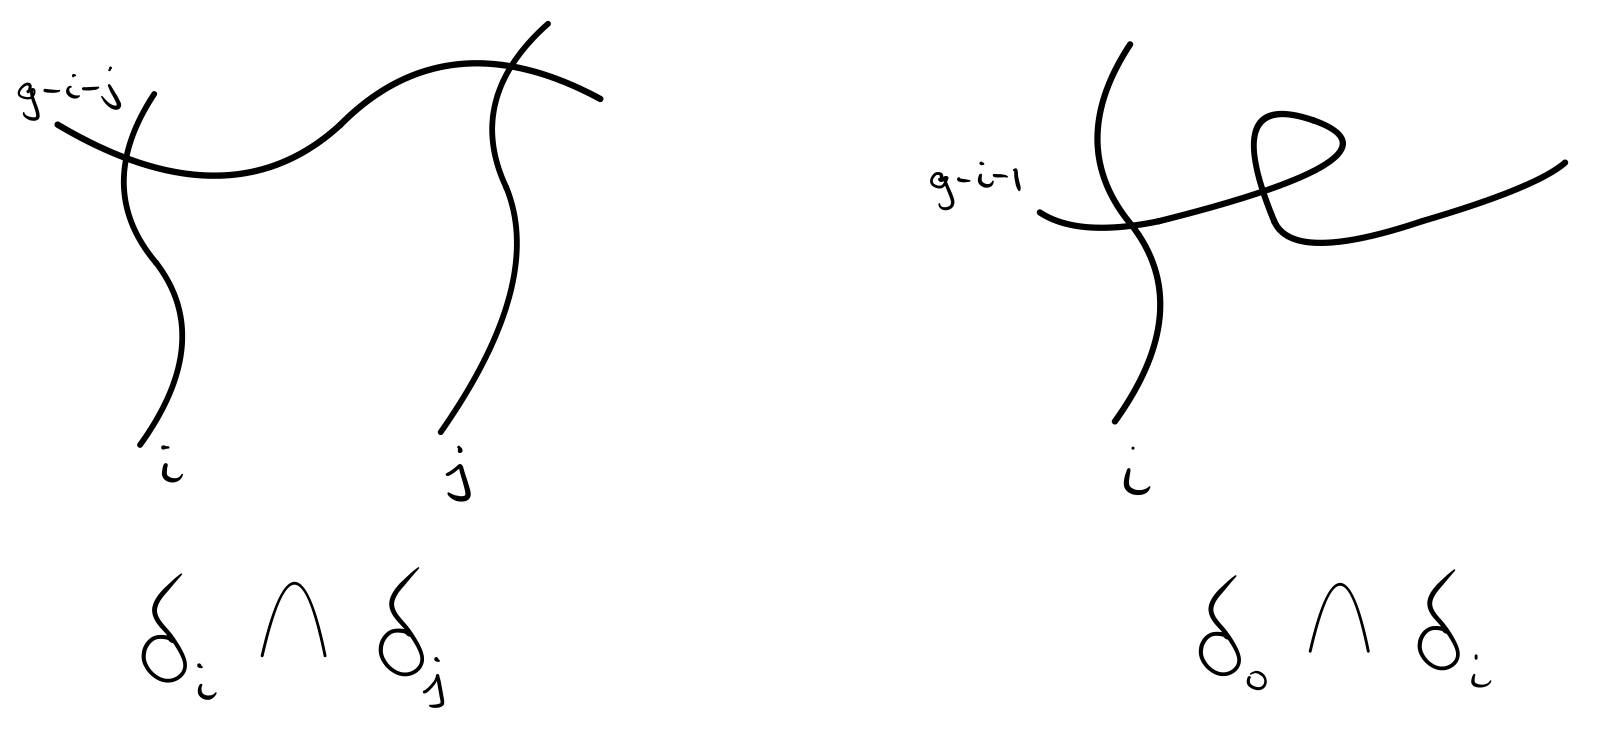
\includegraphics[width=.7\textwidth]{figures/fig-6.7.31.png}
\caption{边界除子 $\delta_i$ 与 $\delta_j$ 的交非空.}\label{src:6.7.31}\end{figure}
\begin{remark}[容许覆盖]\label{src:6.7.32}
上述论证受到 Harris 和 Mumford~\cite{HM82} 为计算 $\overline M_g$ 的 Kodaira 维数而引入的容许覆盖理论的启发. 另见~\cite[\S3.G]{HM98}. 容许覆盖推广单分歧覆盖 $C\to\mathbb P^1$, 允许源曲线和靶曲线具有结点. 其思想是定义模叠 $\overline{\mathcal{Hur}}_{g,\allowbreak b}$, 使其纳入图
\[
\begin{tikzcd}[column sep=small]
&\overline{\mathcal{Hur}}_{g,b}\arrow[dl]\arrow[dr]&\\
\overline{\mathcal M}_g&&\overline M_{0,b}
\end{tikzcd}
\quad\xleftarrow{\text{紧化}}\quad
\begin{tikzcd}[column sep=small]
&\operatorname{Hur}_{g,b}\arrow[dl]\arrow[dr]&\\
\mathcal M_g&&M_{0,b}.
\end{tikzcd}
\]
亏格 $g$ 的\newterm{容许覆盖}{admissible cover} 是从预稳定亏格 $g$ 曲线到稳定 $b$-点亏格 $0$ 曲线 $(B,\allowbreak p_1,\allowbreak \ldots,\allowbreak p_b)$ 的满射有限态射 $f:C\to\allowbreak B$, 满足:
\begin{enumerate}[(a)]
\item $B^{\mathrm{sm}}$ 的原像是 $C^{\mathrm{sm}}$, 诱导态射 $C^{\mathrm{sm}}\to\allowbreak B^{\mathrm{sm}}$ 为在 $p_i$ 上方单分歧的 $d$ 次覆盖, 即分歧指数均为 $2$, 每个纤维至多含一个分歧点;
\item 对每个结点 $q\in B$ 及其上方的每个结点 $r\in C$, $C\to\allowbreak B$ 在 $r$ 处的平展局部结构为 $k[x,\allowbreak y]/(xy)\to\allowbreak k[x,\allowbreak y]/(xy)$, 由 $(x,\allowbreak y)\mapsto(x^m,\allowbreak y^m)$ 定义; 即两个分支在结点处的分歧指数相等.
\end{enumerate}
定义推广到族, 给出固有 Deligne--Mumford 叠 $\overline{\mathcal{Hur}}_{g,\allowbreak b}$. (容许覆盖可有非平凡自同构群, 故此叠不是概形.) 对应 $(C\to\allowbreak B)\mapsto(B,\allowbreak p_i)$ 定义到 $\overline M_{0,\allowbreak b}$ 的态射. 对应 $(C\to\allowbreak B)\mapsto C^{\mathrm{st}}$ 定义到 $\mathcal M_g^{\mathrm{pre}}$ 的态射, 注意源曲线不必稳定. 与稳定收缩态射 (\bookref{6.6.7}) 复合, 得到到 $\overline{\mathcal M}_g$ 的态射.

可用此语言重写命题~\bookref{6.7.26} 的论证. 对 $d\gg0$ 和光滑曲线 $C$, 选取原像 $(C\to\mathbb P^1)\in\operatorname{Hur}_{g,\allowbreak b}$ (引理~\bookref{6.7.16}). 令 $H$ 为包含它的连通分支, $\overline H\subseteq\overline{\mathcal{Hur}}_{g,\allowbreak b}$ 为闭包. 因为 $\operatorname{Hur}_{g,\allowbreak b}\to\allowbreak M_{0,\allowbreak b}$ 有限平展, $\overline H$ 满射到 $\overline M_{0,\allowbreak b}$. 如命题~\bookref{6.7.26} 的证明选择交换图
\[
\begin{tikzcd}
T\setminus\{t\}\arrow[r]\arrow[d]&\overline H\arrow[d,"\text{固有}"]\\
T\arrow[r,"{t\mapsto(D,d_i)}"']&\overline M_{0,b},
\end{tikzcd}
\]
其中 $T$ 光滑连通, $t$ 映到图~\bookref{6.7.27} 的曲线, 某个 $t'\ne t$ 映到 $(C'\to\mathbb P^1)\in H$. 由固有性的赋值判据, 将 $T$ 换为分歧覆盖后, 存在提升 $T\to\overline H$, $t$ 映到容许覆盖 $(C''\to\allowbreak D)$. 如前证明, $C''$ 的每个光滑不可约分支的亏格为 $0$. 所以 $C'$ 退化为有奇点稳定曲线 $(C'')^{\mathrm{st}}$; 原覆盖与 $C'$ 的覆盖同处 Hurwitz 空间的一个连通分支, 故原曲线 $C$ 也退化为它. (构造覆盖族 $\mathcal C\to\mathcal D\to\allowbreak T$ 的论证也是证明容许覆盖叠固有性的关键步骤之一.)
\end{remark}
\subsection{正特征下的不可约性}\label{src:6.7.5-subsection}
遵循 Deligne--Mumford~\cite{DM69} 和 Fulton~\cite{Ful69} 的历史论证, 证明正特征下 $\overline{\mathcal M}_g$ 不可约. 核心是 Zariski 连通性定理 (\bookref{5.6.15}): 对 Noether Deligne--Mumford 叠之间的平坦固有态射, 纤维的几何连通分支数下半连续. 此定理在~\cite[定理 4.17]{DM69} 中陈述但未证明, 所需 Deligne--Mumford 叠理论之多令人惊讶.
\begin{theorem}[$\overline{\mathcal M}_{g,\allowbreak n}$ 的不可约性]\label{src:6.7.33}
若 $2g-2+n>0$, 则 $\overline{\mathcal M}_{g,\allowbreak n}$ 在任意域上不可约.
\end{theorem}
\begin{proof}
由定理~\bookref{6.7.19} 的超越证明或定理~\bookref{6.7.30} 的代数证明, 已知特征 $0$ 的情形, 只需证 $\overline{\mathbb F}_p$ 上的不可约性. 态射 $\overline{\mathcal M}_{g,\allowbreak n}\to\Spec\mathbb Z$ 光滑 (定理~\bookref{6.4.16}) 且固有 (定理~\bookref{6.5.23}), 故 Zariski 连通性定理 (\bookref{5.6.15}) 保证所有几何纤维的连通分支数相同. 由 $\overline{\mathbb Q}$ 上连通, 得到 $\overline{\mathbb F}_p$ 上连通, 从而不可约.
\end{proof}
\begin{remark}[Deligne 和 Mumford 的证明]\label{src:6.7.34}
上面是 Deligne 和 Mumford~\cite[\S5]{DM69} 给出的第二个论证. 请记住, 正是这篇非凡论文引入了叠 (今称 Deligne--Mumford 叠), 引入稳定曲线并证明稳定约化. 第一个不可约性论证~\cite[\S3]{DM69} 被他们称为``该定理的初等推导'', 与定理~\bookref{6.7.30} 利用光滑曲线的退化和边界的归纳结构的证明十分相近. 它依赖稳定约化与 $\mathcal M_g$ 的拓扑不可约性. 下面概述他们对任意域 $k$ 上不可约性的论证.

令 $H_g$ (分别地, $\overline H_g$) 为 $\operatorname{Hilb}^P(\mathbb P_{\mathbb Z}^{5g-6}/\mathbb Z)$ 中参数化光滑 (分别地, 稳定) 曲线的局部闭子概形. Mumford 在~\cite[定理 5.11, 7.13]{GIT} 中将 $\Spec\mathbb Z$ 上粗模概形 $M_g$ 构造为几何商 $H_g/\operatorname{PGL}_{5g-6}$, 并证明它对每个素数 $p$ 在 $\Spec\mathbb Z[1/p]$ 上拟射影. ($\overline{\mathcal M}_g$ 也有 $\Spec\mathbb Z$ 上的射影粗模概形 $\overline M_g$, 可认同为 $\overline H_g/\operatorname{PGL}_{5g-6}$, 但这是后来才证明的.)

\textbf{步骤 $1$: $M_g\times_{\mathbb Z}k$ 无在 $k$ 上固有的连通分支.}
令 $W(k)$ 为 $k$ 的 Witt 向量环; 它是完备 Noether 局部环, 一般点 $\eta$ 的特征为 $0$, 闭点 $0$ 的剩余域为 $k$. (例如 $W(\mathbb F_p)=\mathbb Z_p$ 是 $p$-进数环.) 由于 $M_g\times_{\mathbb Z}W(k)$ 拟射影, 可选包含它作为稠密开子概形的射影紧化
\[
\begin{tikzcd}
M_g\times_{\mathbb Z}W(k)\arrow[r,hook]\arrow[dr]&X\arrow[d,"\text{射影}"]\\
&\Spec W(k).
\end{tikzcd}
\]
由特征 $0$ 的结果, 一般纤维 $X_\eta$ 连通. $X$ 在 $W(k)$ 上平坦固有, 故概形的 Zariski 连通性定理 (\bookref{5.6.15}) 保证特殊纤维 $X_0$ 连通.

假设 $Y\subseteq M_g\times_{\mathbb Z}k$ 是 $k$ 上固有的连通分支. 它在 $X_0$ 中既开, 又因固有而闭. 由 $X_0$ 连通, $Y$ 必为整个 $M_g\times_{\mathbb Z}k$, 故后者固有且不可约. 为得矛盾, 令 $A_{g,\allowbreak k}$ 为主极化 $g$ 维阿贝尔簇模空间, 考虑将光滑曲线映为 Jacobian 的态射 $\Theta:M_g\times_{\mathbb Z}k\to\allowbreak A_{g,\allowbreak k}$, $C\mapsto\operatorname{Jac}(C)$. 固有性意味着像闭, 但当时已知像的闭包包含低维 Jacobian 的乘积.

\textbf{步骤 $2$: $\overline H_g\times_{\mathbb Z}k$ 无完全由光滑曲线组成的连通分支.}
令 $\overline H_g^{(1)},\allowbreak \ldots,\allowbreak \overline H_g^{(r)}$ 为其连通分支. 步骤 $1$ 保证每个 $H_g^{(i)}:=\overline H_g^{(i)}\cap(H_g\times_{\mathbb Z}k)$ 不固有. 因而有不延拓到 $\Delta=\Spec k[[t]]$ 的态射 $\Delta^*=\Spec k((t))\to\allowbreak H_g^{(i)}$. 由稳定约化 (\bookref{6.5.1}), 必要时将 $\Delta$ 换为分歧扩张后, 它延拓为 $\Delta\to\overline H_g^{(i)}$. 因而 $\overline H_g^{(i)}\setminus H_g^{(i)}$ 非空. 换言之, 每条光滑曲线退化为有奇点稳定曲线, 给出命题~\bookref{6.7.26} 的正特征证明.

\textbf{步骤 $3$: 边界 $\delta\times_{\mathbb Z}k$ 连通, 其中 $\delta=\overline M_g\setminus M_g$.}
由步骤 $2$, 后者蕴涵 $\overline M_g\times_{\mathbb Z}k$ 连通. 证明各 $\delta_i\times_{\mathbb Z}k$ 连通, 且每个两两交非空. 这正是定理~\bookref{6.7.30} 的证明利用亏格归纳, 粘合态射和图~\bookref{6.7.31} 中曲线所做的事. Deligne 和 Mumford 基本上给出相同论证, 但采用针对性技巧, 因为 $n$-点稳定曲线模空间与粘合态射的形式体系是 Knudsen 后来才引入的.

有趣的是, 两个证明均不本质依赖叠理论. 只要知道存在固有平坦的粗模空间 $\overline M_{g,\allowbreak n}\to\Spec\mathbb Z$, 第二个证明便成立. 但两个证明都根本依赖紧化 $\overline{\mathcal M}_g$ 与稳定约化.
\end{remark}
\begin{remark}[Fulton 的证明]\label{src:6.7.35}
Fulton~\cite{Ful69} 研究参数化在 $b$ 个无序点上方单分歧的 $d$ 次覆盖族 $\mathcal C\to\mathbb P^1_S$ 的变体 $\operatorname{Hur}_{g,\allowbreak b}^{\mathrm{rig,\allowbreak unord}}$ (见注记~\bookref{6.7.12}), 证明图
\[
\begin{tikzcd}
&\operatorname{Hur}_{g,b}^{\mathrm{rig,unord}}\arrow[dl]\arrow[dr,"\text{平展}"]&\\
\mathcal M_g&&\operatorname{Sym}^b\mathbb P^1\setminus\Delta=\mathbb P^b\setminus\Delta
\end{tikzcd}
\]
在 $\mathbb Z$ 上定义, 且 $d\geq g+1$ 时左方映射满射 (比推论~\bookref{6.7.18} 的界更好), 右方到 $M_{0,\allowbreak n}$ 的映射在 $\mathbb Z_{d!}$ 上有限平展, 即倒置所有素数 $p\leq d$ 后如此. Fulton 建立了``约化定理'': 若 $X$ 是完备离散赋值环 $R$ 上的光滑射影概形, $R$ 的剩余域 $k$ 代数闭, 分式域 $K$ 的特征为 $0$, $\Delta\subseteq X$ 是单纯相对除子 (即每个纤维无多重分支), 且有限平展覆盖 $Y\to\allowbreak X\setminus\Delta$ 满足 $Y_{\overline K}$ 不可约, 则 $Y_k$ 也不可约. 利用特征 $0$ 下 Hurwitz 空间不可约, 将此定理应用于 $\operatorname{Hur}_{g,\allowbreak b}^{\mathrm{rig,\allowbreak unord}}\to\operatorname{Sym}^b\mathbb P^1\setminus\Delta$, 得到特征 $p>d$ 下的不可约性. 取 $d=g+1$, 得到特征 $p>g+1$ 下 $\mathcal M_g$ 不可约.
\end{remark}
